\section{Simulation of the selected strategies}
\label{sc:simofstrat}
\head{This section contains simulations and verifications of the previously selected formation control strategies separated in steps from initial structure to complete formation control.}
\subsection{The potential field strategy}
The theory of potential fields are implemented with the strategy proposed in section \ref{sc:potential-fields}. The potential field is generated for each individual agent at every update step to make the formation move and converge to a specified formation and position. The field is generated based on forces acting in a overlying potential field structure where one force converges the agent to a desired position, a force attracting the agent to obtain the desired formation along the trajectory, a force repelling the agent from other agents is their distance is too small and finally a force repelling the agents from static objects. The latter two can seem the same, but the repelling force will be larger for the agent-agent force due to the fact that two agents could have course directly toward each other and a more aggressive avoidance can be needed.

To be able to generate and simulate the potential field then implementation needs to be generic. First it was developed with one agent that needs to converge to a desired position and afterwards were other agents added as obstacles and some static objects were added in extend. From these obstacles it can be seen that a single agent are able to converge to a position which makes it possible to expand such that more agents can converge into formation with reference from either a virtual leader or from each other. This will solve the formation coordination task, where the following task will be the group coordination task. The group coordination task has the goal to move the formation around, which here will be done by making the virtual leader, or an actual leader of the formation, follow a trajectory specified. This will make the other agents follow this leader and withhold their formation on the trajectory.
\begin{figure}[htbp]
  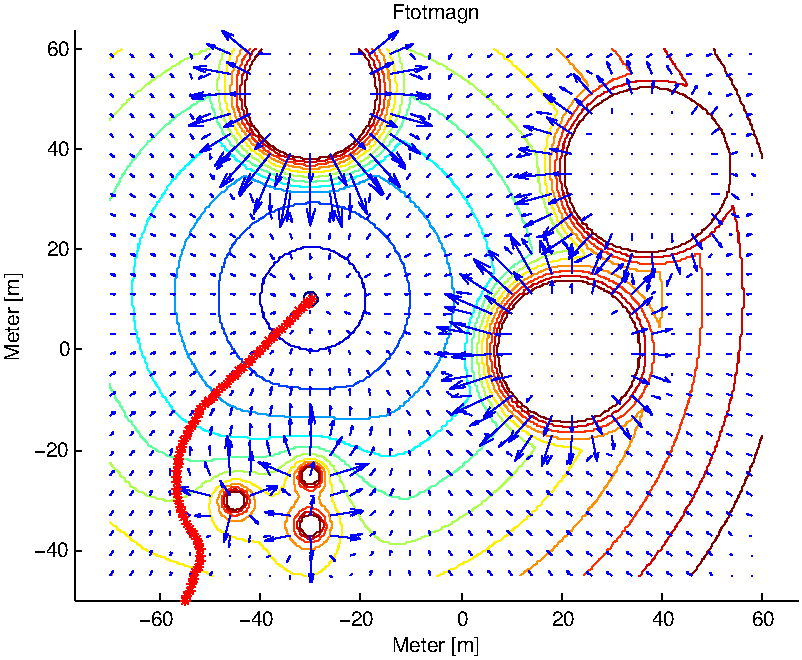
\includegraphics[width=0.9\textwidth]{fig/ftotmagnfigpdf1}
  \caption{Plot of one agent's trajectory with a desired position with obstacles to avoid}
  \label{fig:potfieldagenti}
\end{figure}
A plot for a total potential reference field for a single agent can be seen on figure \ref{fig:potfieldagenti}. The red line made of crosses are the trajectory that one single agent will follow, if the obstacles to avoid in the plot are static. In the plot every object, either an other agent or an object, are kept static. So it shows how the trajectory will be in one single time step. This will change in the next time step if the other agents also move in the potential field. In this specific plot is a safety radius ($r$) of $20$m chosen, such that the distance from agent $p_i$ (The red trajectory) to any obstacle always will be larger than $20$m.
This radius applies both to other agents seen in the following equation
\[
    F_{ca}^{ij}= 
\begin{cases}
    \frac{K_{ca}r}{||d_{ij}||}-K_{ca},& \text{for } ||d_{ij}||<r\\
    0,              & \text{otherwise}
\end{cases}
\]
and to obstacles seen in the following equation
\[
    F_{oa}^{ik}= 
\begin{cases}
    \frac{K_{oa}}{||d_{ki}||}-\frac{K_{oa}}{r},& \text{for } ||d_{ki}||<r\\
    0,              & \text{otherwise}
\end{cases}
\]
where the gains $K_{ca}$ and $K_{oa}$ are chosen equally to a constant as 240. If this gain is chosen smaller it will result in that the agents are more allowed to approach the obstacles and get a little within the radius, but then afterwards getting repelled from the object. It corresponds to the gradient at the radius and how steep this is.

The gain of $K_{ij}$ is not to be interpret from figure \ref{fig:potfieldagenti}. $K_{ij}$ is the gain to the force that attracts the agents together by minimizing the distance in between them. By doing this the agents will get faster into the desired formation. The gain $K_{vl}$ does at some point the opposite. This gain adjusts the weighting of how fixated the agents should be to converge to the desired position. If this gain is relatively larger than $K_{ij}$ then the agents will converge directly to their position around the virtual leader and not converge to the desired formation on the way. This implies that the scaling between $K_{vl}$ and $K_{ij}$ controls if the formation should converge to the desired formation on the way to desired position, or if agent $i$ should only have the desired position in focus.

The grid in which the potential field is generated are limited with a certain resolution while simulating the agents movement. This reduces the directions of where the agents can move, which will not arise a problem on the same level when implemented in reality. In the simulation environment it reduces the resolution such that a single field in the grid contains one value of magnitude of the potential field, which makes the basis of a certain gradient to the field. The agents are following the implementation of the steepest decent. This generates a gradient towards the steepest decent, which makes the agent track this. The analogy can be seen as a bowl, or sphere in this case, where a ball will converge towards the lowest point in the direction of the minimum gradient.

The method of applying the grid with magnitude of the potential field arises the problem with resolution, but also a problem that makes the 'corners' of the grid around the agent to be more likely to have the steepest decent. This problem has been expanded with a solution such that a certain radius around an agent will be checked. The value at the radius around the agent can be checked, and due to the equal distance to every point, these will be weighted equally with respect to their value. This makes the possibility to in principle make the agent go in all directions which will be closer to the reality. When testing the two methods against each other it is clear that the first proposed with the grid structure did not have the same mobility thus not preferable though simpler.

Another problem that can become crucial arises when two objects are within the radius of each other. This will result in a local minima in the potential field between those objects. If an agent converges toward this minima they cannot get out again. The problem can be seen on figure \ref{fig:roevproblem}. The gains here are chosen exactly the same as in figure \ref{fig:potfieldagenti}.
\begin{figure}[htbp]
  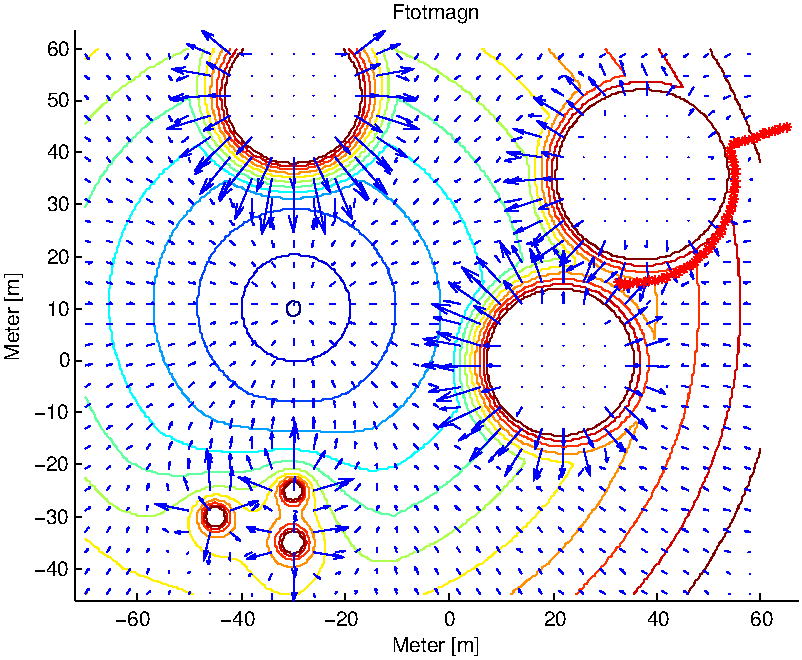
\includegraphics[width=0.9\textwidth]{fig/ftotmagnfigpdf3}
  \caption{An agent gets stuck due to a local minima between two other agents. The agent cannot get out of this minima unless the other two agents makes the space for the agent to pass through}
  \label{fig:roevproblem}
\end{figure}
Solutions to this problem can be formulated in different ways. One solution could be to cluster the two objects together and instead of making their potential field individually, then combine those together and make an ellipsoid or even a circle formed obstacle of those objects. This will ensure that the local minima disappears thus not making an agent get stuck between those objects.

In the end this results in that the every agent needs a magnitude and a direction of which they should move. This will be given depending on the total environment where the agents are manoeuvring. When applying this formation strategy a collision free movement are guaranteed which is one of the more critical criteria to be fulfilled. \todo{Det her skal der nok skrives lidt matematik om som viser det, eller en god forklaring. Men dog er det jo en naturlig del af pot field.}

\subsection{Adding the Dynamics for Simulation}
\todo{Should this be moved to the potentialfield.tex?}
Describe the block diagram connecting the potential field calculations,
an analogy to the wp\_gen script for the path follower.

Describe how the dynamics will affect the trajectory.

Describe the behaviour when a boat gets stuck in a local minima. hhjj

\begin{figure}[htbp]
\centering
\includesvg{potentialfield_block}
\caption{Block diagram showing the iteration process of using the
potential fields for computation of the input vector}
\label{fig:potentialfield_block}
\end{figure}

The potential field control system consists of multiple elements
as seen with the e flow is illustrated on the block diagram on
figure~\vref{fig:potentialfield_block}.

Part og this flow can be computed by the $i$'th ship themselves.


The implementation of this is tested in matlab, using the m-files;

potfield.m, pathgen.m, shipcontroller.m, simaauship.m

The simulation algorithm for the multiship potential field should keep
in mind that shall save the timeseries for the ship states, the
control inputs and the local reference trajectory for the $i$'th ship.

Ignoring the initialization of all the variables, the outer loop
guidance navigation and control algorithm using potential fields are
as follows.

The \ac{GNC} works by an array of mission specific way points given,
usually computed from a desired area used to create a lawnmower
pattern described in chapter~\vref{ch:pathgen} describing the path
generation.

\paragraph{Global Trajectory Generation}
Then different methods can be used to steer ships after this
trajectory. The simplest is the usual heading autopilot, which will
just steer the reading of the ship to the course angle to the
way point. Or more elaborate, ways is the use of the way points as
linesegments that the ship should follow. This is implemented with a
\ac{LOS} algorithm. This algorithm, can work, but it is too simple to
include obstacle or inter vehicle collisions. A way proposed to solve
this issue is to use the concept of potential fields.

\paragraph{Potential Field}
The potential field itself is merely some functions describing the
repulsive and repelling forces between points of interest in the map.
These points of interest are all objects that matters for the
navigation, that is all ships, the anchor point (virtual leader) of
the formation, and other point obstables. This using the methodology
described in the paper \citep{UAVff3dpf}.

The potential field is used in an iterative algorithm which can
calculate the direction (from the $i$'th boat to the desired position
spaned by a potential field defining the formation.

\paragraph{Local Trajectory Generation}
In the end, a reference path is calculated by the means of the
previous previous position and the result from the potential field
solver. It is calculated as the paper presents, \citep[eq.
48]{UAVff3dpf}.

\begin{align}
	\mathbf{p}_{i,r}^n = \mathbf{p}_i^n + \mathbf{F}_i ^\text{tot}
\end{align}

This is passed to the ships inner control loop.

